
\begin{figure*}
	\centering
	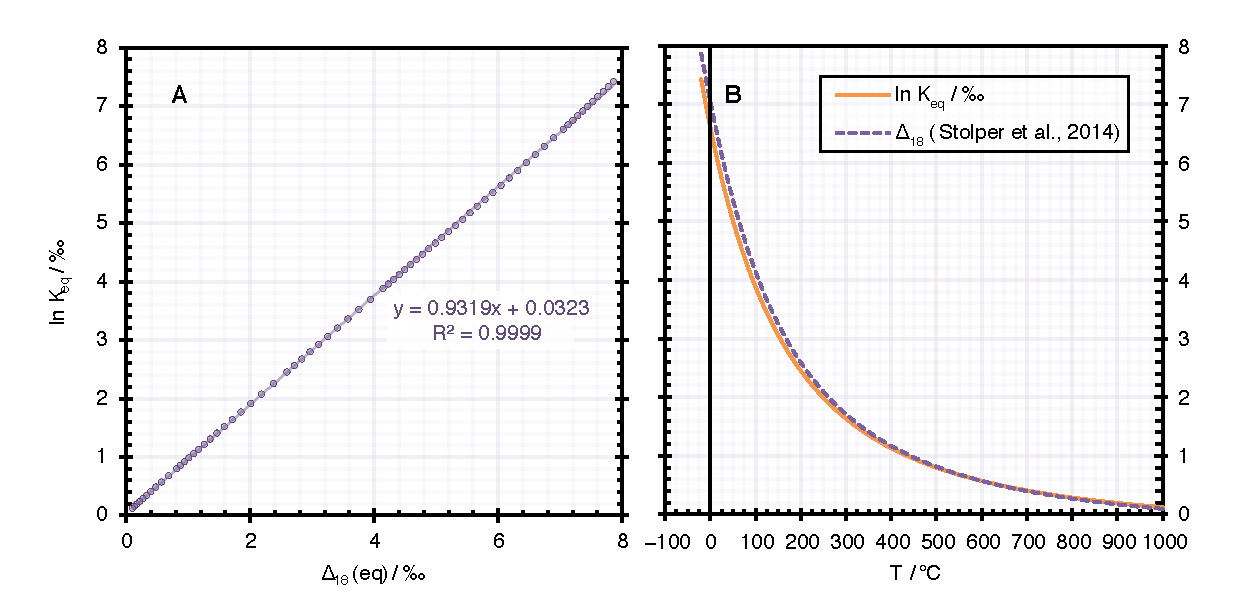
\includegraphics[width=\textwidth]{figures/FigC.2}
	\captionsetup{format=myformat}	% hrule beneath caption
	\caption[Equilibrium Δ\textsubscript{18} and Δ\textsuperscript{13}CH\textsubscript{3}D values as a function of temperature]{Equilibrium Δ vs.\ $T$ curves.  (\textbf{A}) Conversion between equilibrium
		Δ\textsubscript{18} values and equilibrium
		Δ\textsuperscript{13}CH\textsubscript{3}D values. Note that conversion
		of Δ\textsubscript{18} to Δ\textsuperscript{13}CH\textsubscript{3}D can
		only be done if it is known or can be assumed that methane isotopologues
		have attained their equilibrium distribution at the temperature
		indicated by both Δ\textsuperscript{13}CH\textsubscript{3}D and Δ\textsuperscript{12}CH\textsubscript{2}D\textsubscript{2}. Nonequilibrium
		Δ\textsubscript{18} values cannot easily be converted to
		Δ\textsuperscript{13}CH\textsubscript{3}D, particularly if Δ \textless{}
		0 ‰ (anticlumped). (\textbf{B}) Comparison between equilibrium
		Δ\textsuperscript{13}CH\textsubscript{3}D [= ln
		\emph{K}\textsubscript{eq} for the isotope exchange reaction (\autoref{eqn:C:exchange}), defined
		following \textcite{Ono++_2014_AC} and calculated as in \textcite{Wang++_2015_S}], and equilibrium Δ\textsubscript{18}
		values from \textcite{Stolper++_2014_GCA}.}
	\label{fig:C:2}
\end{figure*}